\documentclass[11pt]{article}

\usepackage[colorlinks=true]{hyperref}
\usepackage{afterpage}
\usepackage{enumerate}

% This is a toggle for whether the solutions should be included in output of this document
\newif\ifSolutions
%\Solutionsfalse  % this is used to exclude the solutions
\Solutionstrue  % this is used to include the solutions


\usepackage[left=0.8in, right=0.8in, top=0.7in, bottom=1in, includefoot]{geometry}
\usepackage{fancyhdr}
\usepackage{array}
\usepackage{multicol}
\setlength{\parindent}{0mm}
\setlength{\parskip}{5pt}
\usepackage{sectsty}
\allsectionsfont{\sffamily}
\setlength{\headheight}{2cm}
\usepackage{amsmath,amssymb,bm}
\usepackage{booktabs}
\usepackage{graphicx}
\usepackage{color}
\usepackage{cancel}
\usepackage{comment}
\usepackage{hyperref}
\usepackage{subfig}
\usepackage{multirow}
\usepackage{placeins}

% Global definitions
%
% boldface letters
%
%\newcommand{\boldface}[1]{\mathbf{#1}}   % upright
\newcommand{\boldface}[1]{\boldsymbol{#1}}  % italic (slanted)
%
\newcommand{\bfa}{\boldface{a}}
\newcommand{\bfb}{\boldface{b}}
\newcommand{\bfc}{\boldface{c}}
\newcommand{\bfd}{\boldface{d}}
\newcommand{\bfe}{\boldface{e}}
\newcommand{\bff}{\boldface{f}}
\newcommand{\bfg}{\boldface{g}}
\newcommand{\bfh}{\boldface{h}}
\newcommand{\bfi}{\boldface{i}}
\newcommand{\bfj}{\boldface{j}}
\newcommand{\bfk}{\boldface{k}}
\newcommand{\bfl}{\boldface{l}}
\newcommand{\bfm}{\boldface{m}}
\newcommand{\bfn}{\boldface{n}}
\newcommand{\bfo}{\boldface{o}}
\newcommand{\bfp}{\boldface{p}}
\newcommand{\bfq}{\boldface{q}}
\newcommand{\bfr}{\boldface{r}}
\newcommand{\bfs}{\boldface{s}}
\newcommand{\bft}{\boldface{t}}
\newcommand{\bfu}{\boldface{u}}
\newcommand{\bfv}{\boldface{v}}
\newcommand{\bfw}{\boldface{w}}
\newcommand{\bfx}{\boldface{x}}
\newcommand{\bfy}{\boldface{y}}
\newcommand{\bfz}{\boldface{z}}
%
\newcommand{\bfA}{\boldface{A}}
\newcommand{\bfB}{\boldface{B}}
\newcommand{\bfC}{\boldface{C}}
\newcommand{\bfD}{\boldface{D}}
\newcommand{\bfE}{\boldface{E}}
\newcommand{\bfF}{\boldface{F}}
\newcommand{\bfG}{\boldface{G}}
\newcommand{\bfH}{\boldface{H}}
\newcommand{\bfI}{\boldface{I}}
\newcommand{\bfJ}{\boldface{J}}
\newcommand{\bfK}{\boldface{K}}
\newcommand{\bfL}{\boldface{L}}
\newcommand{\bfM}{\boldface{M}}
\newcommand{\bfN}{\boldface{N}}
\newcommand{\bfO}{\boldface{O}}
\newcommand{\bfP}{\boldface{P}}
\newcommand{\bfQ}{\boldface{Q}}
\newcommand{\bfR}{\boldface{R}}
\newcommand{\bfS}{\boldface{S}}
\newcommand{\bfT}{\boldface{T}}
\newcommand{\bfU}{\boldface{U}}
\newcommand{\bfV}{\boldface{V}}
\newcommand{\bfW}{\boldface{W}}
\newcommand{\bfX}{\boldface{X}}
\newcommand{\bfY}{\boldface{Y}}
\newcommand{\bfZ}{\boldface{Z}}

\newcommand{\bfFe}{\boldface{F}_{\text{e}}}
\newcommand{\bfFp}{\boldface{F}_{\text{p}}}
\newcommand{\bfepse}{\pmb{\varepsilon}_{\text{e}}}
\newcommand{\bfepsp}{\pmb{\varepsilon}_{\text{p}}}
\newcommand{\bfeps}{\pmb{\varepsilon}}

%
% boldface greek symbols
%
\newcommand{\bfalpha}{\boldsymbol{\alpha}}
\newcommand{\bfbeta}{\boldsymbol{\beta}}
\newcommand{\bfgamma}{\boldsymbol{\gamma}}
\newcommand{\bfdelta}{\boldsymbol{\delta}}
\newcommand{\bfepsilon}{\pmb{\varepsilon}}
\newcommand{\bfzeta}{\boldsymbol{\zeta}}
\newcommand{\bfeta}{\boldsymbol{\eta}}
\newcommand{\bftheta}{\boldsymbol{\theta}}
\newcommand{\bfkappa}{\boldsymbol{\kappa}}
\newcommand{\bflambda}{\boldsymbol{\lambda}}
\newcommand{\bfrho}{\boldsymbol{\rho}}
\newcommand{\bfmu}{\boldsymbol{\mu}}
\newcommand{\bfnu}{\boldsymbol{\nu}}
\newcommand{\bfpi}{\boldsymbol{\pi}}
\newcommand{\bfxi}{\boldsymbol{\xi}}
\newcommand{\bfsigma}{\boldsymbol{\sigma}}
\newcommand{\bftau}{\boldsymbol{\tau}}
\newcommand{\bfphi}{\boldsymbol{\phi}}
\newcommand{\bfvarphi}{\boldsymbol{\varphi}}
\newcommand{\bfchi}{\boldsymbol{\chi}}
\newcommand{\bfomega}{\boldsymbol{\omega}}
\newcommand{\bfnull}{\boldsymbol{0}}
%
\newcommand{\bfGamma}{\boldsymbol{\Gamma}}
\newcommand{\bfDelta}{\boldsymbol{\Delta}}
\newcommand{\bfTheta}{\boldsymbol{\Theta}}
\newcommand{\bfLambda}{\boldsymbol{\Lambda}}
\newcommand{\bfPi}{\boldsymbol{\Pi}}
\newcommand{\bfXi}{\boldsymbol{\Xi}}
\newcommand{\bfSigma}{\boldsymbol{\Sigma}}
\newcommand{\bfPhi}{\boldsymbol{\Phi}}
\newcommand{\bfChi}{\boldsymbol{\Chi}}
\newcommand{\bfOmega}{\boldsymbol{\Omega}}
\newcommand{\bfnabla}{\boldsymbol{\nabla}}
\newcommand{\laplace}{\boldsymbol{\Delta}}
%
% caligraphic letters
%
\newcommand{\calA}{\mathcal{A}}
\newcommand{\calB}{\mathcal{B}}
\newcommand{\calC}{\mathcal{C}}
\newcommand{\calD}{\mathcal{D}}
\newcommand{\calE}{\mathcal{E}}
\newcommand{\calF}{\mathcal{F}}
\newcommand{\calG}{\mathcal{G}}
\newcommand{\calH}{\mathcal{H}}
\newcommand{\calI}{\mathcal{I}}
\newcommand{\calJ}{\mathcal{J}}
\newcommand{\calK}{\mathcal{K}}
\newcommand{\calL}{\mathcal{L}}
\newcommand{\calM}{\mathcal{M}}
\newcommand{\calN}{\mathcal{N}}
\newcommand{\calO}{\mathcal{O}}
\newcommand{\calP}{\mathcal{P}}
\newcommand{\calQ}{\mathcal{Q}}
\newcommand{\calR}{\mathbb{R}}
\newcommand{\calS}{\mathcal{S}}
\newcommand{\calT}{\mathcal{T}}
\newcommand{\calU}{\mathcal{U}}
\newcommand{\calV}{\mathcal{V}}
\newcommand{\calW}{\mathcal{W}}
\newcommand{\calX}{\mathcal{X}}
\newcommand{\calY}{\mathcal{Y}}
\newcommand{\calZ}{\mathcal{Z}}
% .. define more if needed
%
% double stroke
%
\newcommand{\dsA}{\mathbb{A}}
\newcommand{\dsB}{\mathbb{B}}
\newcommand{\dsC}{\mathbb{C}}
\newcommand{\dsD}{\mathbb{D}}
\newcommand{\dsE}{\mathbb{E}}
\newcommand{\dsF}{\mathbb{F}}
\newcommand{\dsG}{\mathbb{G}}
\newcommand{\dsH}{\mathbb{H}}
\newcommand{\dsI}{\mathbb{I}}
\newcommand{\dsJ}{\mathbb{J}}
\newcommand{\dsK}{\mathbb{K}}
\newcommand{\dsL}{\mathbb{L}}
\newcommand{\dsM}{\mathbb{M}}
\newcommand{\dsN}{\mathbb{N}}
\newcommand{\dsO}{\mathbb{O}}
\newcommand{\dsP}{\mathbb{P}}
\newcommand{\dsQ}{\mathbb{Q}}
\newcommand{\dsR}{\mathbb{R}}
\newcommand{\dsS}{\mathbb{S}}
\newcommand{\dsT}{\mathbb{T}}
\newcommand{\dsU}{\mathbb{U}}
\newcommand{\dsV}{\mathbb{V}}
\newcommand{\dsW}{\mathbb{W}}
\newcommand{\dsX}{\mathbb{X}}
\newcommand{\dsY}{\mathbb{Y}}
\newcommand{\dsZ}{\mathbb{Z}}



\newcommand{\vect}[1]{\mathbf{#1}}
\newcommand{\grvect}[1]{\mbox{\boldmath{$#1$}}}
\newcommand{\perm}{\mbox{{\Huge $\epsilon$}}}
\newcommand{\transvect}[1]{\vect{#1}^{\mbox{\footnotesize T}}}
\newcommand{\invvect}[1]{\vect{#1}^{\mbox{\footnotesize -1}}}
\newcommand{\partderiv}[2]{\frac{\partial #1}{\partial #2}}
\newcommand{\partderivv}[2]{\frac{\partial^2 #1}{\partial #2^2}}
\newcommand{\totalderiv}[2]{\frac{d #1}{d #2}}

\newcommand{\mg}[1]{{\boldsymbol{#1}}}
\newcommand{\mf}[1]{{\mathfrak{#1}}}
\newcommand{\mfb}[1]{{\boldsymbol{\mathfrak{#1}}}}
\newcommand{\ms}[1]{{\mathscr{#1}}}
\newcommand{\mb}[1]{{\mathbf{#1}}}
\newcommand{\mbb}[1]{{\mathbb{#1}}}
\newcommand{\mbbu}[1]{{\underline{\mathbb{#1}}}\vphantom{#1}}
\newcommand{\mbu}[1]{{\underline{\mathbf{#1}}}\vphantom{#1}}
\newcommand{\mgu}[1]{{\underline{\boldsymbol{#1}}}\vphantom{#1}}
\newcommand{\mr}[1]{{\mathrm{#1}}}
\newcommand{\msf}[1]{{\mathsf{#1}}}
\newcommand{\msfb}[1]{{\boldsymbol{\mathsf{#1}}}}

\newcommand{\dotprod}{\stackrel{\scriptscriptstyle \bullet}{}}
\newcommand{\half}{\frac{1}{2}}
\newcommand{\T}{^{\mathsf{T}}} % x^{T}
\newcommand{\mT}{^{\mathsf{-T}}} % x^{-T}
\newcommand{\wass}{\mathsf{wass}}
\newcommand{\eff}{\mathsf{eff}}
\newcommand{\me}{^{\mathrm{-1}}} % x^{-1}
\newcommand{\Rset}{\ensuremath{\mathbb{R}}}
\newcommand{\Kset}{\ensuremath{K}}
\newcommand{\bul}{$\bullet\;$}
%\newcommand{\red}{\mathrm{red}}
\newcommand{\Fe}{\mathbf{F}_\mathbf{e}}
\newcommand{\Fp}{\mathbf{F}_\mathbf{p}}
\def\rel{{\mathrm{rel}}}

%\newcommand{\D}{\displaystyle}
\newcommand{\abs}{\rule[-1cm]{0cm}{1cm}}
\newcommand{\babs}{\rule[-1cm]{0cm}{2cm}}

\newlength{\boxwidth}
\setlength{\boxwidth}{\textwidth}
\addtolength{\boxwidth}{-1cm}

\newcommand\pl{\partial}
\def\dd{\;\!\mathrm{d}}
\def\DD{\;\!\mathrm{D}}
\def\Lin{\R^{d\times d}} 
\def\R{I\!R}
\def\AM{{\mathrm{AM}}}

\def\btheorem{\begin{theorem}}
\def\etheorem{\end{theorem}}
\def\blemma{\begin{lemma}}
\def\elemma{\end{lemma}}
\def\bproposition{\begin{proposition}}
\def\eproposition{\end{proposition}}
\def\bcorollary{\begin{corollary}}
\def\ecorollary{\end{corollary}}
\def\bdefinition{\begin{definition}}
\def\edefinition{\end{definition}}
\def\bexample{\begin{example}}
\def\eexample{\end{example}}
\def\bremark{\begin{remark}}
\def\eremark{\end{remark}}
\def\bproblem#1{\medskip \noindent {\bf #1}\sl \\ }
\def\eproblem{\rm \medskip}
\newcommand{\bma}{ \left( \ba}
\newcommand{\ema}{ \ea \right)}
\newcommand{\set}[2]{\big\{\: #1 \: \big| \: #2 \:\big\} }
\def\cD{\mathcal{D}}
\def\cL{\mathcal{L}}
\def\cG{\mathcal{G}}
\def\cI{\mathcal{I}}
\def\cJ{\mathcal{J}}
\def\ccA{\mathcal{A}}
\def\rmD{\mathrm{D}}
\def\bbQ{\mathbb{Q}}
\def\bbA{\fg{A\!\!\!A}}
\def\fg{\boldsymbol}
\def\mdot{\fg{:}}
\def\vdot{\fg{\cdot}}
\newcommand{\el}{\mathsf{el}}
\def\id{{\bfI}}
\def\eqldef{{\:{\stackrel{\mathrm{def}}{=}}\:}}
\newcommand{\eps}{\varepsilon}
\def\ol{\overline}
\def\wt{\widetilde}
\def\wh{\widehat}
\def\ds{\displaystyle}
\def\ts{\textstyle}
\def\mtr{^\mathrm{-T}}
\def\inh{^\mathrm{inh}}
\DeclareMathOperator{\divv}{div}
\DeclareMathOperator{\grad}{grad}
\DeclareMathOperator{\tr}{tr}
\DeclareMathOperator{\curl}{curl}
\DeclareMathOperator{\Curl}{Curl}
%\DeclareMathOperator{\T}{T}
\DeclareMathOperator{\argmin}{{arg\,min}}
\DeclareMathOperator{\diag}{diag}
\DeclareMathOperator{\trace}{tr}
\DeclareMathOperator{\sign}{sign}
\DeclareMathOperator{\dev}{dev}
\DeclareMathOperator{\cof}{cof}
\DeclareMathOperator{\sym}{sym}
\DeclareMathOperator{\skews}{skw}
\def\Felast{\bfF_\mathbf{\!e}}
\def\Fplast{\bfF_\mathbf{\!p}}
\def\Cplast{\bfC_\mathbf{\!p}}
\def\epselast{\bfeps_\mathbf{\!e}}
\def\epsplast{\bfeps_\mathbf{\!p}}
\def\GLin{\mbox{{\sf GL}$(d)$}}  %{\R^{d\times d}_*}% invertible matrices
\def\Lin{\R^{d\times d}}        % all d times d matrices
\def\reff#1{(\ref{#1})}
\def\red{{\mathrm{red}}}
\def\rep{{\mathrm{rep}}}
\def\cond{{\mathrm{cond}}}
\newcommand{\kopfcolor}{\color{red}}
\newcommand{\er}{\hspace*{4cm}}
\newcommand{\n}{{\rm n}}
\newcommand{\nn}{{\rm n+1}}
\newcommand{\PsiS}{\Psi_\mathrm{S}}
\newcommand{\PsiV}{\Psi_\mathrm{V}}
\newcommand{\PsiI}{\Psi_\mathrm{I}}
\newcommand{\cA}{c_\mathrm{A}}
\newcommand{\cM}{c_\mathrm{M}}

\newcommand{\calAe}{\underset{e=1}{\overset{n_e}{\mathcal{A}}}}
\newcommand{\Grad}{\text{Grad}}
\newcommand{\tcr}{\tau_{\text{crit}}}
\newcommand{\be}{\begin{equation}\nonumber}
\newcommand{\ee}{\end{equation}}
\newcommand{\beq}{\begin{eqnarray}}
\newcommand{\eeq}{\end{eqnarray}}
\newcommand{\bem}{\begin{multline}}
\newcommand{\eem}{\end{multline}}
\newcommand{\ba}{\begin{align}}
\newcommand{\ea}{\end{align}}
\newcommand{\bfzero}{{\fg0}}

\renewcommand{\figurename}{Figure}
\renewcommand{\tablename}{Table}

\newcommand{\fp}[2]{\frac{\partial #1}{\partial #2} }
\newcommand{\LR}{{\qquad \Leftrightarrow \qquad }}
\newcounter{problem}
\newcounter{points}
\newcounter{stretchPoints}

\newcommand{\head}[3]{

\begin{center}
\section*{Homework Set \##1 \ifSolutions Solutions \fi}
assigned: #2\\
due: #3, 11:00 pm\\
in your repo at /cs/cs181j/2015/fall/students/your\_user\_name/cs181j \\
\end{center}
\hrule
\vskip 0.1cm
}

\newcommand{\prob}[1]{\par\vskip 0.5cm \stepcounter{problem}\subsubsection*{Problem \arabic{problem} \ \small (#1 points).}\addtocounter{points}{#1}}
\newcommand{\total}{
\begin{flushright}
\small\par\vskip 0.3cm \textit{total: \arabic{points} points ({\color{blue}+\arabic{stretchPoints} stretch points})}
\end{flushright}
}

\newcommand{\eprob}[2]{\par\vskip 0.5cm \stepcounter{problem}\subsubsection*{Problem \arabic{problem}: #2 \ \small (#1 points).}\addtocounter{points}{#1}}

\newcommand{\estretchprob}[3]{\par\vskip 0.5cm \stepcounter{problem}\subsubsection*{Problem \arabic{problem}: #3 \ \small (#1 points ({\color{blue}+#2 stretch points}) ).}\addtocounter{points}{#1}\addtocounter{stretchPoints}{#2}}


%\endinput

\usepackage{afterpage}
\usepackage{enumerate}

\begin{document}
\sffamily
\pagestyle{fancy}
\renewcommand{\headrulewidth}{0.4pt}
\fancyfoot[C]{\sffamily \thepage{}}
\fancyhead[C]{\vskip 0.7cm \sffamily\footnotesize \textbf{cs181j -- High Performance Computing} \hfill \name\\ Fall 2015 \hfill Harvey Mudd College}

% Convenience function used for including a figure
\newcommand\Figure[3]
{
    \begin{figure}[h!]
        \begin{center}
    \includegraphics[width=#3 in]{#1}
    \caption{\label{fig:#1} {#2}}
    \end{center}
    \end{figure}
}

\newcommand\TwoFigure[7]
{
    \begin{figure}[h!]
        \subfloat[#2]{\includegraphics[width=#7 in]{#1}}
    \hfill
        \subfloat[#4]{\includegraphics[width=#7 in]{#3}}
        \caption{\label{fig:#6}#5}
    \end{figure}
}

\newcommand\TwoFigureVertical[7]
{
    \begin{figure}[h!]
        \subfloat[#2]{\includegraphics[width=#7 in]{#1}}

        \subfloat[#4]{\includegraphics[width=#7 in]{#3}}
        \caption{\label{fig:#6}#5}
    \end{figure}
}


\fancyhead[RL]{}

%\newcommand{\name}{I forgot to change my name}


\head{13}{Friday, December 11, 2015}{\href{https://www.youtube.com/watch?v=kfVsfOSbJY0t=45}{Friday}, December 18, 2015}

In this homework assignment, you'll parallelize a simplistic 2D \textbf{molecular dynamics} simulation using \href{http://www.open-mpi.org/doc/v1.8/}{MPI} and produce something that looks like \href{https://www.youtube.com/watch?v=\_4cFGOkoSoI}{this}. 
As discussed in class, in general you can parallelize in one of two paradigms: \textbf{``Big Picture''} where everyone sees the big picture or \textbf{``Need to Know''}, where each process actually only has a subset of the domain.  
On this assignment, you'll do both techniques.

The way that the particles interact is not important (and it's totally bogus, by the way), but the data that is needed to update particle positions is important.  
In particular, in order to calculate the new position of each particle on a given timestep, you need to know the previous position and velocity of all particles within some cutoff distance, and you need the previous position, velocity, and acceleration of the particle you're updating.

Serial implementations are provided for you.  
I'll need you to provide \textbf{movies} for this assignment; I cannot tell if it's working without movies, so upload them to youtube or somehow make them available to me.  
The code has a tunable parameter named \texttt{stickingTimescale}, which can be used to determine how much the particles stick to each other when they collide.  
You can change this for fun, but your movies must be made at the \texttt{stickingTimescale} that I provide in the starting code.

Don't try to make these implementations super efficient by hiding communication cost or anything, just get them working.  
They won't even necessarily go any faster than the serial versions because the problem is just so absurdly, unbelievably small.  
However, egregiously inefficient implementations, such as all processes communicating with all other processes or processes sending each other way more messages than necessary (where one or two would be sufficient), will receive lower grades.

{
  \begin{figure}[h!]
    \begin{center}
    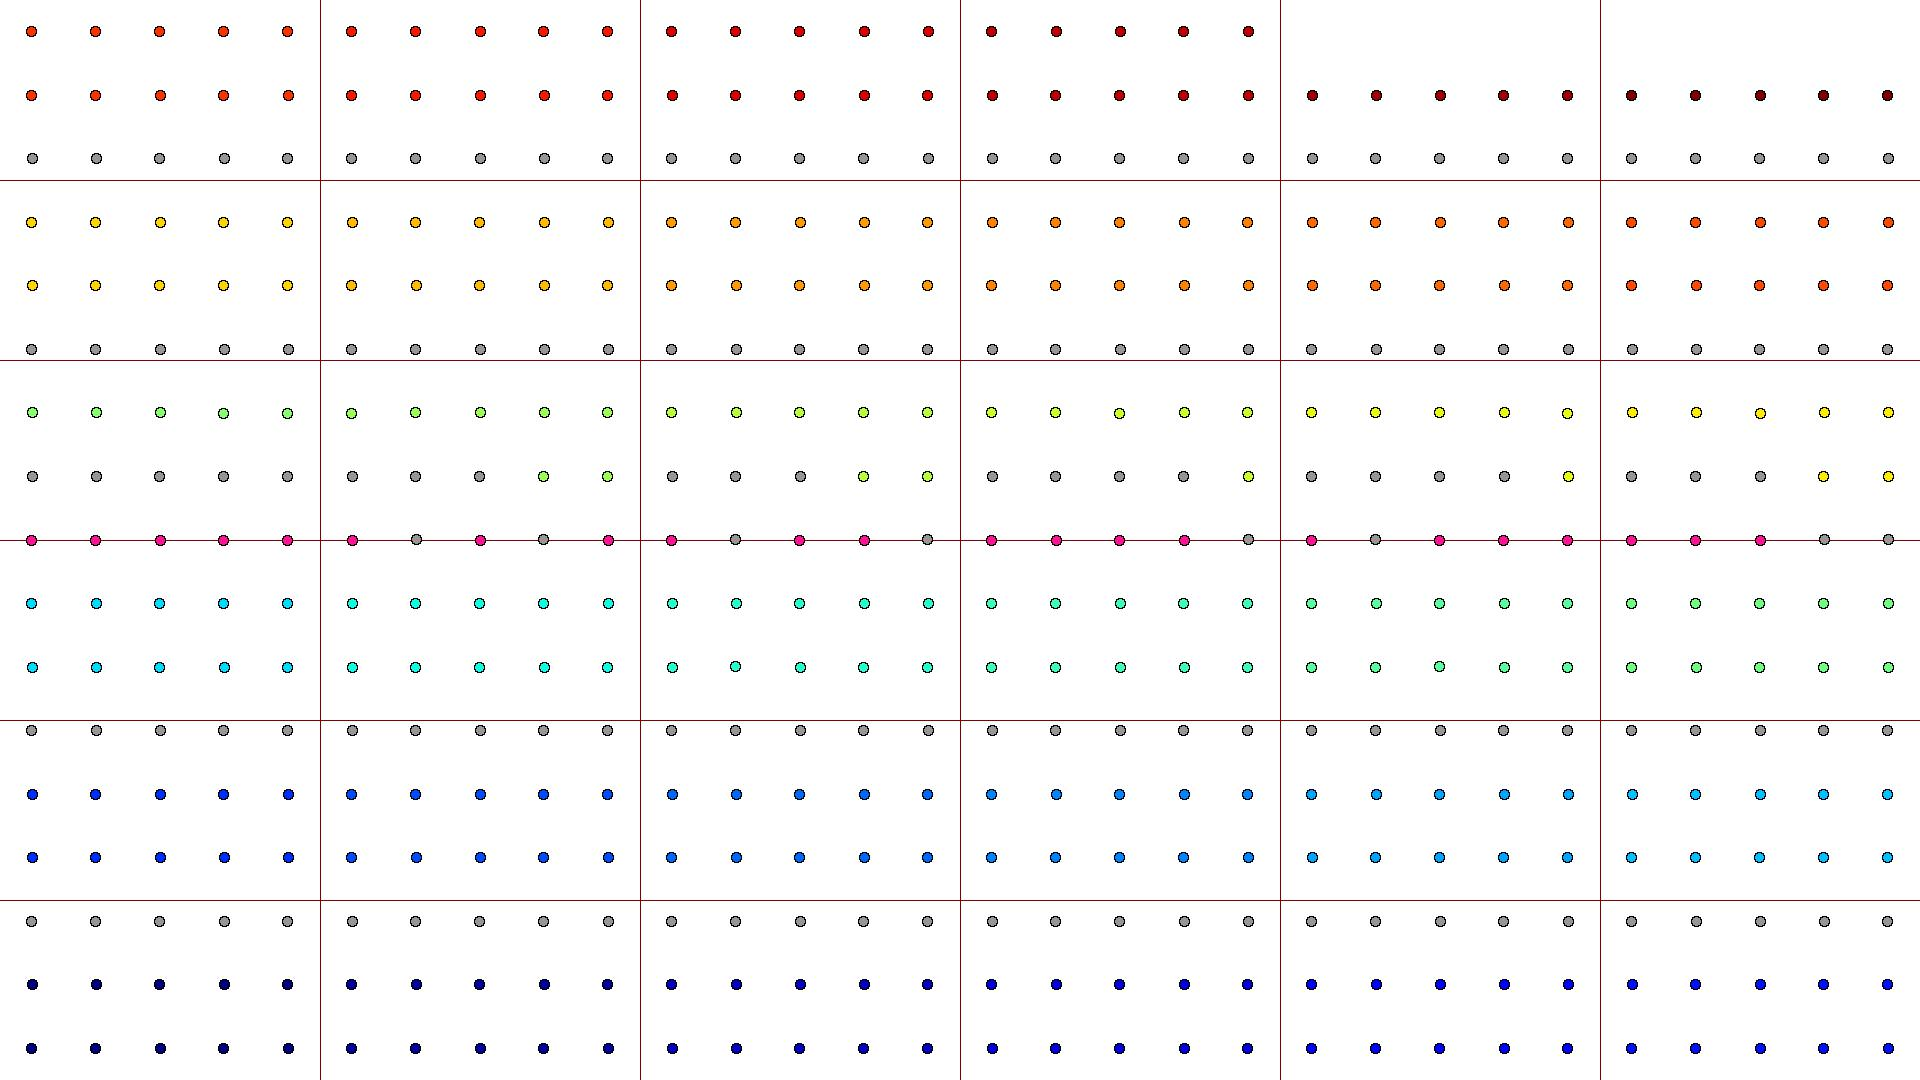
\includegraphics[width=6.0 in]{Mini2dMD_NeedToKnow_036_00000}
    \end{center}
    \caption{Initial State}
    \label{fig:InitialState}
  \end{figure}
}
{
  \begin{figure}[h!]
    \begin{center}
    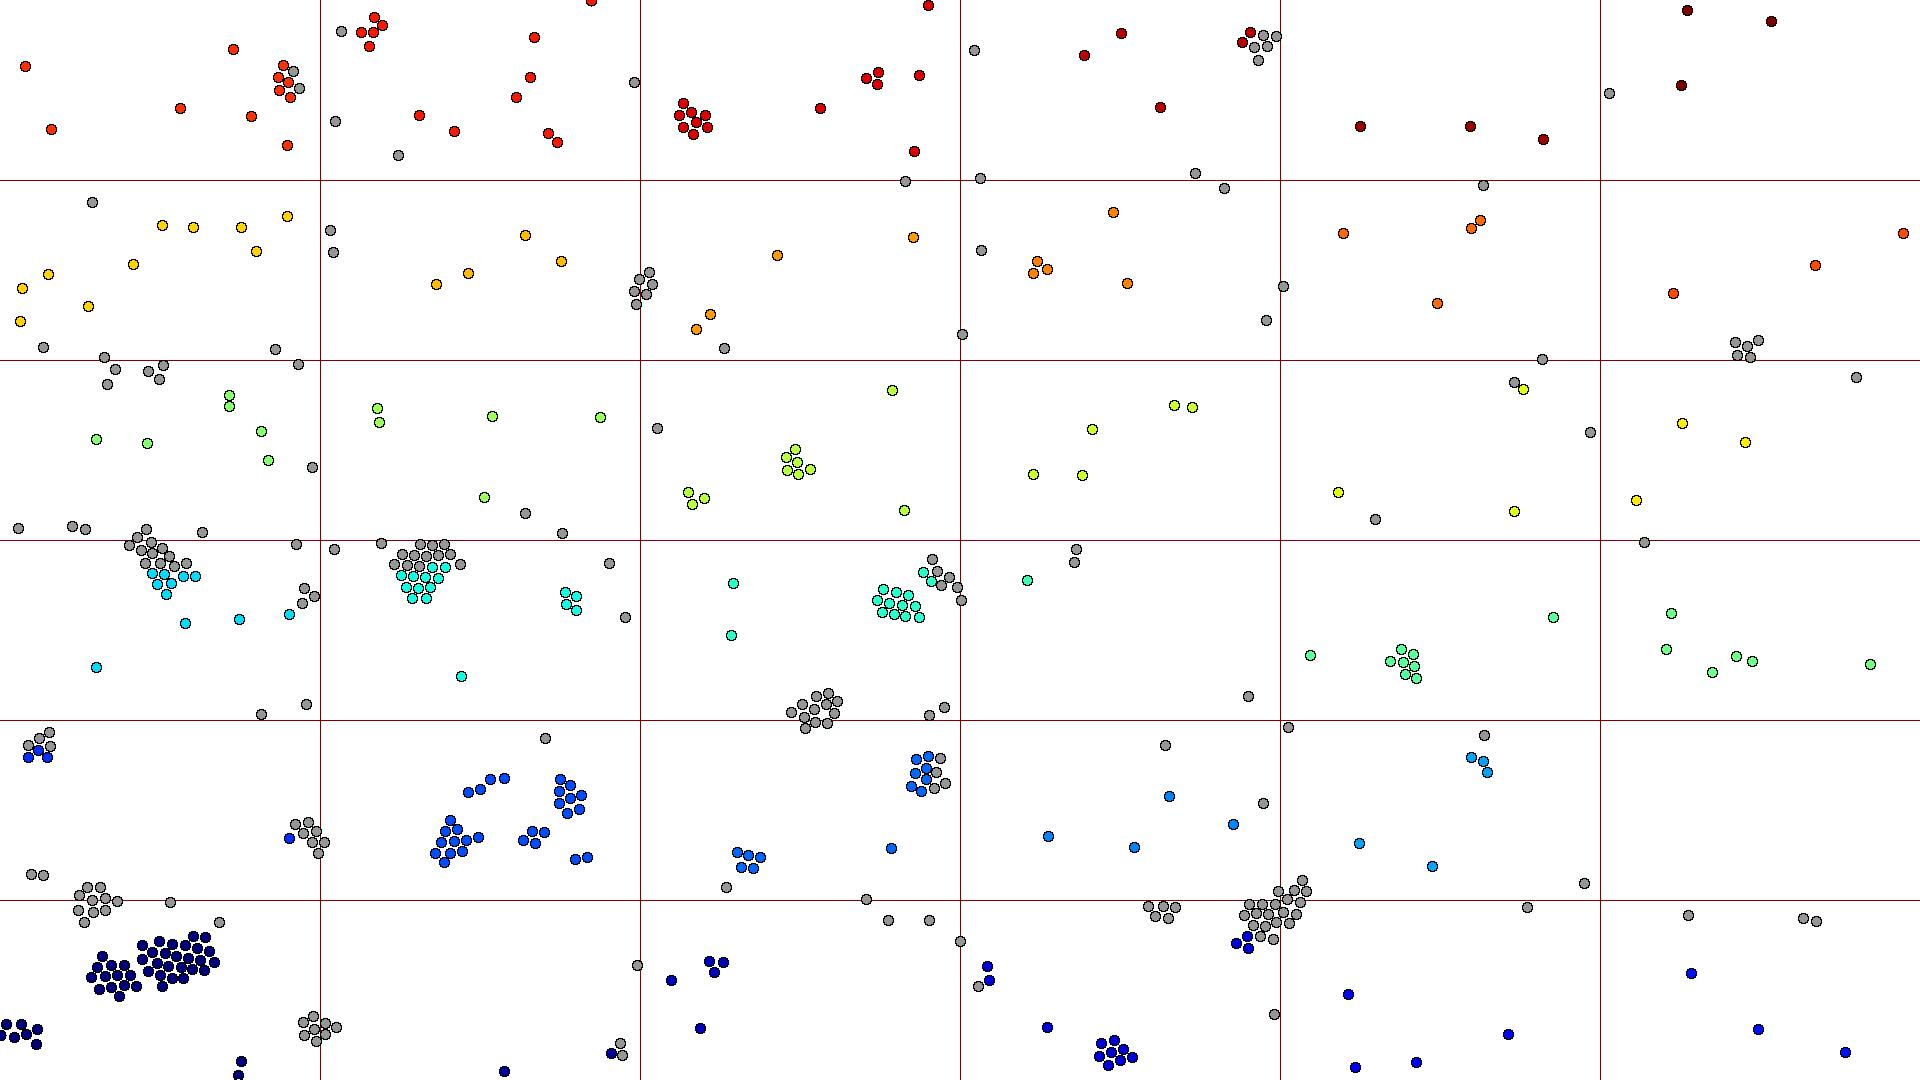
\includegraphics[width=6.0 in]{Mini2dMD_NeedToKnow_036_00079}
    \end{center}
    \caption{Intermediate State}
    \label{fig:IntermediateState}
  \end{figure}
}
{
  \begin{figure}[h!]
    \begin{center}
    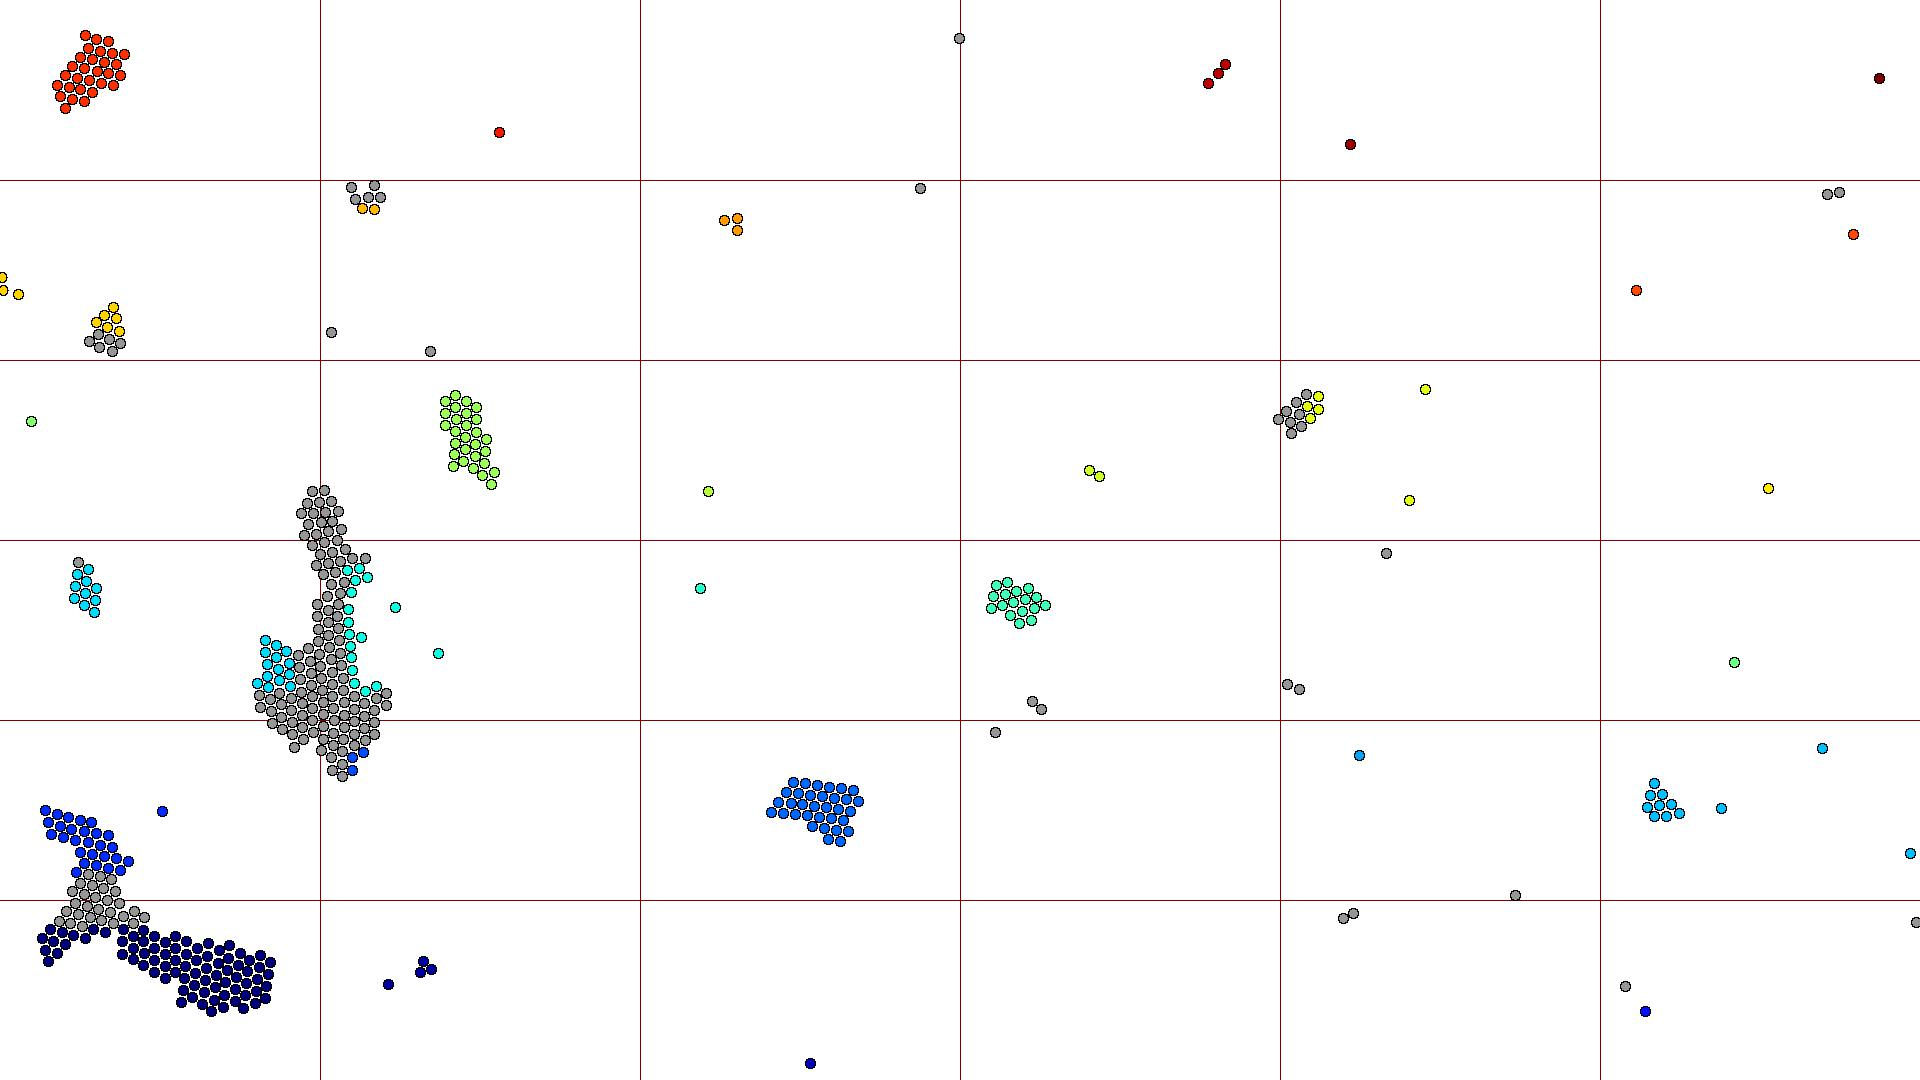
\includegraphics[width=6.0 in]{Mini2dMD_NeedToKnow_036_00249}
    \end{center}
    \caption{Final State}
    \label{fig:FinalState}
  \end{figure}
}

\afterpage{\clearpage}











\eprob{25}{Big Picture}

Parallelize the MD solver with ``Big Picture'' parallelism.

\begin{enumerate}[a)]
\item (10 points) Describe in pseudocode the ``Big Picture'' version of the code, including what MPI functions you would call and what data is stored where.  
Start from the following pseudocode of what's provided:

\textbf{Solution:}

\begin{verbatim}
generate initial positions and velocities for all of the particles in the simulation
vector<Point> positions
vector<Vector> velocities
vector<Vector> accelerations
for each timestep
  find neighbors of all particles
  calculate the force on each particle and average velocity of neighbors
  calculate the new velocity of each particle using the current force,
    the old acceleration, and the old average velocity of neighbors and
    store the new velocity into velocities
  store the acceleration of each particle into accelerations
  calculate the new position of each particle and store into positions
  apply boundary conditions to velocities and positions
  write output file
\end{verbatim}

\item (15 points) Implement the ``Big Picture'' version, make a movie for 20 processes, and make it available to me.

\end{enumerate}

\begin{itemize}
\item \textbf{Note:} this version should get exactly the same answer, regardless of the number of processes used.  
For correctness purposes, make sure that the last frame of the movie looks the same for 1 or (say) 20 processes.
\item There is an expensive black box function to find neighbors so that you don't have to do it.  
Don't modify this function; you don't need to parallelize it for this assignment.
\item The code outputs the magnitude of the total velocity across the entire simulation.  This is just a quick sanity check so that you can know if your current attempt is exploding or not without having to render the thing.
\end{itemize}

\ifSolutions
\textbf{Solution:}

I see the \href{https://www.youtube.com/watch?v=J---aiyznGQ}{big picture}.

\fi

\newpage















\eprob{45}{Need to Know}

Here's the moment you've been waiting for, your chance at the minor leagues: \href{https://youtu.be/LkCNJRfSZBU?t=83}{parallelize} the MD solver with ``Need to Know'' parallelism.  
This is a hard problem.  
You should think hard about and do part a for sure, but only do part b if it's worth the points to you.

\begin{enumerate}[a)]
\item (15 points) Describe in pseudocode the ``Need to Know'' version of the code, including what MPI functions you would call and what data is stored where.  
Note that because it will be difficult for many people to get their ``Need to Know'' version working, I will be using your pseudocode in this problem to determine if you see what needs to be done in order to parallelize the problem.  
I will grade this carefully; be very specific - statements \href{https://www.youtube.com/watch?v=lj3iNxZ8Dww#t=25}{like, such as} ``the process sends data to other processes'' are not sufficient.  
When you are sending something to another rank, be very specific: what are you sending, to whom, with what kind of send?
Start from the following pseudocode of what's provided:

\textbf{Solution:}

\begin{verbatim}
generate initial positions and velocities for all of the particles in the simulation
vector<Point> positions
vector<Vector> velocities
vector<Vector> accelerations
for each timestep
  find neighbors of all particles
  calculate the force on each particle and average velocity of neighbors
  calculate the new velocity of each particle using the current force,
    the old acceleration, and the old average velocity of neighbors and
    store the new velocity into velocities
  store the acceleration of each particle into accelerations
  calculate the new position of each particle and store into positions
  apply boundary conditions to velocities and positions
  write output file
\end{verbatim}

\item (30 points) Implement the ``Need to Know'' version, make a movie for 16 processes, and make it available to me. 

\ifSolutions
\textbf{Solution:}

I have a \href{https://www.youtube.com/watch?v=oKI-tD0L18A&}{need to know}.

\fi

\end{enumerate}

\begin{itemize}
\item If we were implementing a form of this ``Need to Know'' version for an arbitrary number of processes, it would be really hard.
To simplify, require that the number of processes used be a runtime-provided ``square'' such as 9 or 16, so that you can split up the domain into a grid of boxes.  
The solution uses the domain decomposition shown in figure \ref{fig:ShadowRegions}, but you can do whatever you'd like.  
Note: to clarify, you're not hard-coding a certain number of processes, you are just restricting the admissible numbers to 1, 4, 9, 16, 25, 36, etc.  
I will run your code with numbers other than 16 processes.
\item As usual, coordination may be done with collectives, but any data (positions, velocities, accelerations, etc.) must be sent by point-to-point communication, not in collectives.
\item Each rank will have to send shadow particles to its (up to) 8 neighbors.   
However, because the particle position update requires neighbor positions \emph{and} velocities, you'll need to send both positions and velocities to the neighbors.
\item You will need to not only send shadow particles between processes, but when particles leave your rank's boundaries, you'll also have to transfer ownership of particles between processes.  
When you do this, you need to transfer not just the particle position, but also its velocity and acceleration.
\item You may use the \texttt{BoundingBox}'s \texttt{computeBoundaryProximity} function if you'd like; the solution uses it with \texttt{thisRanksBoundingBox} to figure out to which (one or more) of the rank's eight neighbors a given point needs to be shadowed.
\item In the solution, no one rank ever stores the particles in the entire simulation, even during initialization.  
You are allowed to have one rank see the big picture during initialization, but after initialization each rank must only have its individual piece of the problem.
\item The version of MPI on shuffler is compiled such that processes spin while waiting for messages, which means that if you run more processes than the number of cores, each collective communication will take the os thread scheduler's quantum, which means massive slowdowns.  
Don't use more processes than cores, and you'll have to try not to stomp on each others' toes again.
\item In figures \ref{fig:InitialState} through \ref{fig:FinalState}, the particles are painted by their owning rank and shadowed particles are painted grey.  
You do not have to paint your shadow particles grey in your movies.
\item To debug what's happening, it's often nice to be able to draw all of the particles that are on a given rank.  
You can do this by running ``python generateMini2dMDPlots\_NeedToKnow\_Debug.py numberOfProcesses rank''.
You can then make a movie of that one rank's particles by running ``sh MakeMovie\_Debug.sh numberOfProcesses rank''.  
An example movie is \href{http://youtu.be/ci3r1LRTGIM}{here}.  
The format of the output file from which this movie is made is ``x y tag'' for each particle.  
Right now, the tags are all zero because there are no such things as shadow particles in the provided code, and all particles with tag 0 are drawn in the rank's color.  
If you change the tag of a particle to 1 or 2 in the output file, it will be drawn in pink or grey, respectively.  
For example, in the linked movie, particles that we're shadowing to other processes are drawn pink and particles that are being shadowed to this process are drawn in grey.  
\item If your particles are \href{https://www.youtube.com/watch?v=a1Y73sPHKxw}{doing questionable things}, you might find it helpful to increase the number of output files until there is one output file per timestep so that you can see as things start blowing up.
\end{itemize}

\Figure{ShadowRegions}{Domain Decomposition and Shadowing}{4}

\vfill






\eprob{20}{The Real World}

You knew this was coming: answer your technically-adept (they've taken 70, but not 105 or HPC) friend's question ``how do I make my code go fast?'' 
Starting from single-threaded code that uses scalar registers (there is parallelism in single-threaded, scalar code!) and progressing through the class material up to and including message-passing, talk about how to write code that goes fast, what type of parallelism is possible at each stage, how it's leveraged by the programmer, and what potential speedups are possible.

\ifSolutions
\textbf{Solution:}

\fi









\eprob{5}{Course Feedback}

I know that you have already given me very useful (and kind!) feedback. 
The card was so awesome, I really appreciate it.
You were so sneaky.

Can I ask you for one last thing?  
Please fill out the course evaluation found \href{https://docs.google.com/forms/d/1GQPXWXIaeSpAorp_yfRW67a9MHQm94YfMsRpc47LhD0/viewform?usp=send_form}{here}, in which I ask about which technical topics of the class you liked and things like that.

\eprob{5}{Feedback}

\begin{enumerate}[a)]
\item How much total time did you spend on this assignment?
\item Of the total time, how much total time did you spend ``flailing'' on little annoying things that are not the main point of the assignment?
\item Of the total time, how much total time did you spend on the ``Need to Know'' implementation?
\item Did you have any ``aha'' moments where something \href{https://www.youtube.com/watch?v=oHg5SJYRHA0}{clicked}?  If so, on what problems or parts?
\item Can you give me any feedback on this assignment?
\end{enumerate}

\vfill

\vskip 1cm
\total

\end{document}

todo: perform handwriting analysis on student evaluations and prepare grade change forms
